本实验在三个不同的图像对上进行了特征提取与匹配,
分别是 Notre Dame、Mount Rushmore 和 Episcopal Gaudi。
通过proj2.ipynb,我们获得了特征点检测和匹配的可视化结果,并计算了匹配的准确率。

\subsection{可视化结果}
图1-9展示了 Notre Dame, Mount Rushmore图像对的特征匹配结果。

可以看到,SIFT特征成功地在两幅图像之间建立了对应关系,
即使在视角和尺度存在一定差异的情况下。
但是类似的可视化结果在 Mount Rushmore 和 Episcopal Gaudi 图像对没有显现。
\begin{figure}[h!]
    \centering
    \begin{minipage}[b]{0.3\textwidth}
        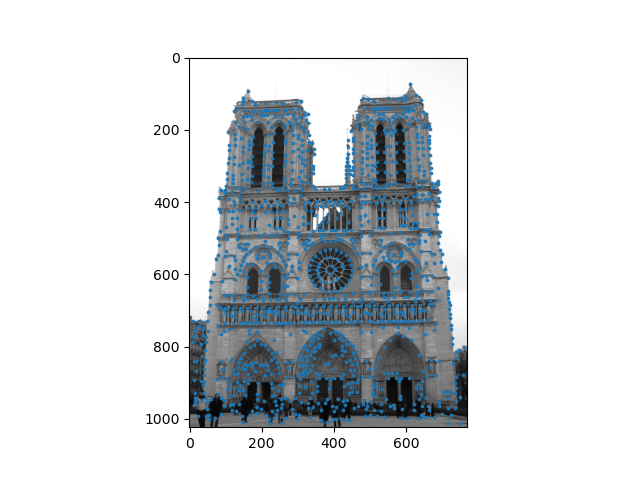
\includegraphics[width=\textwidth]{imgs/notre_dame1.png}
        \caption{Notre Dame 1}
    \end{minipage}
    \begin{minipage}[b]{0.3\textwidth}
        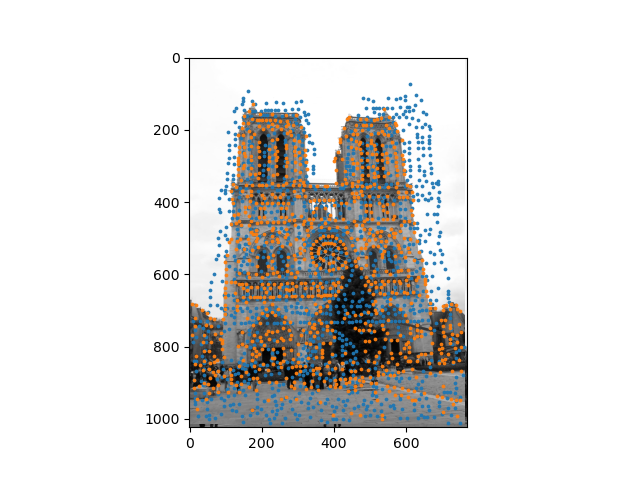
\includegraphics[width=\textwidth]{imgs/notre_dame2.png}
        \caption{Notre Dame 2}
    \end{minipage}
    \begin{minipage}[b]{0.3\textwidth}
        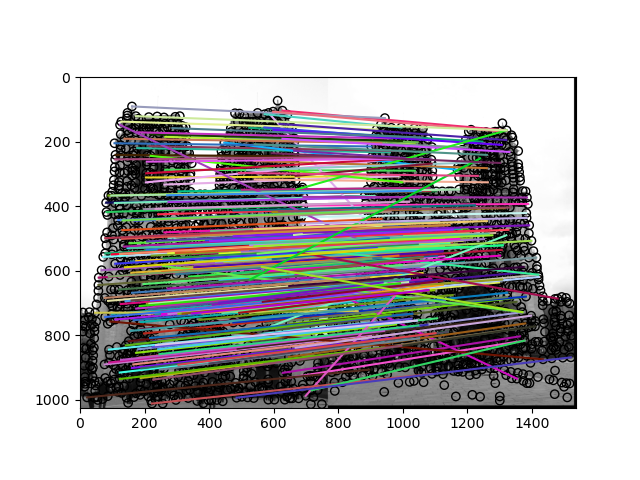
\includegraphics[width=\textwidth]{imgs/notre_dame3.png}
        \caption{Notre Dame match}
    \end{minipage}
    
    \begin{minipage}[b]{0.3\textwidth}
        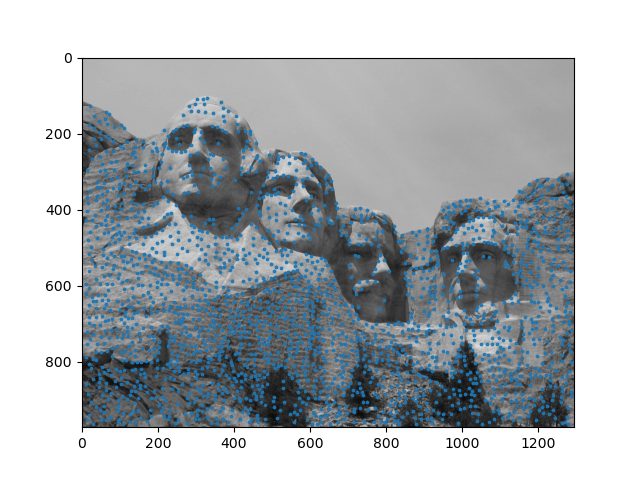
\includegraphics[width=\textwidth]{imgs/mt_rushmore1.png}
        \caption{Mount Rushmore 1}
    \end{minipage}
    \begin{minipage}[b]{0.3\textwidth}
        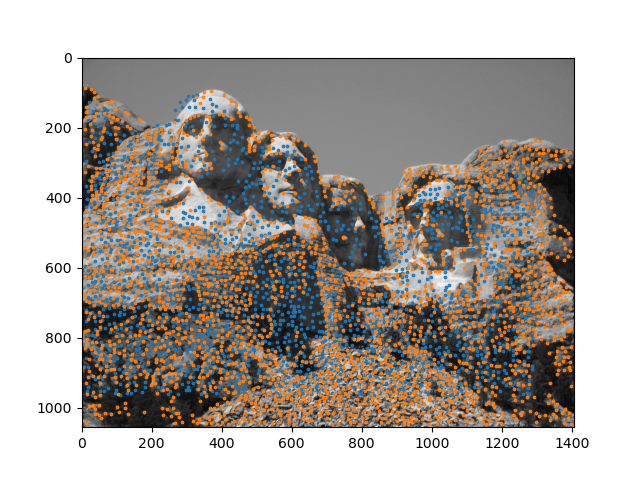
\includegraphics[width=\textwidth]{imgs/mt_rushmore2.png}
        \caption{Mount Rushmore 2}
    \end{minipage}
    \begin{minipage}[b]{0.3\textwidth}
        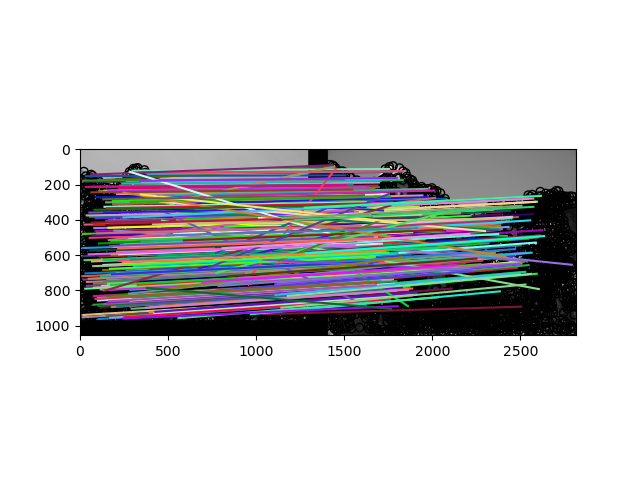
\includegraphics[width=\textwidth]{imgs/mt_rushmore3.png}
        \caption{Mount Rushmore match}
    \end{minipage}
    
    \begin{minipage}[b]{0.3\textwidth}
        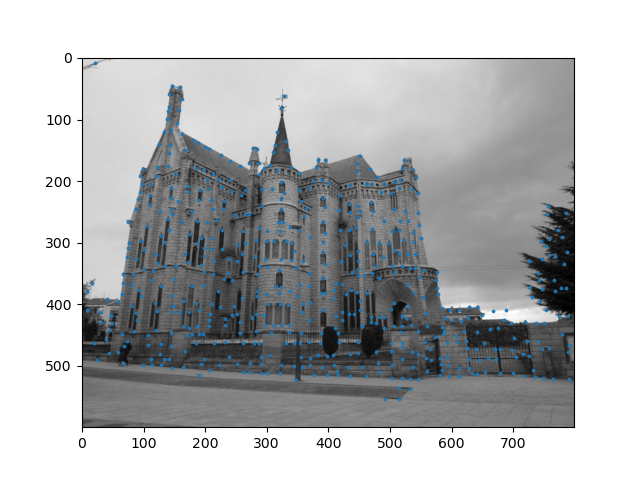
\includegraphics[width=\textwidth]{imgs/e_gaudi1.png}
        \caption{Episcopal Gaudi 1}
    \end{minipage}
    \begin{minipage}[b]{0.3\textwidth}
        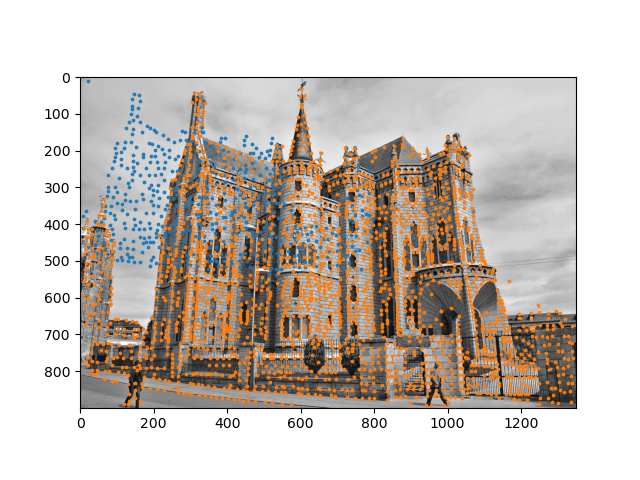
\includegraphics[width=\textwidth]{imgs/e_gaudi2.png}
        \caption{Episcopal Gaudi 2}
    \end{minipage}
    \begin{minipage}[b]{0.3\textwidth}
        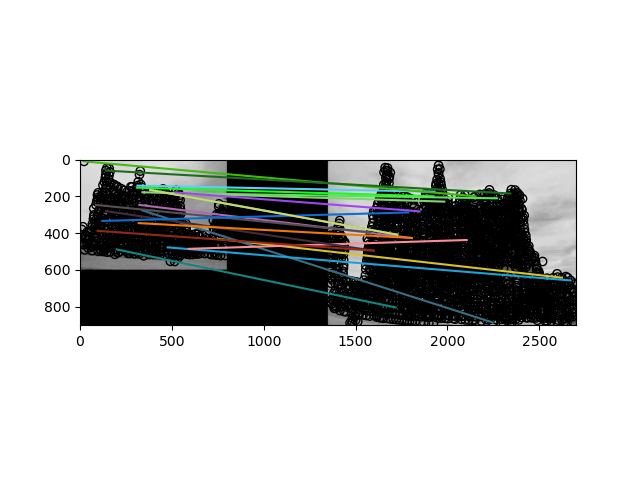
\includegraphics[width=\textwidth]{imgs/e_gaudi3.png}
        \caption{Episcopal Gaudi match}
    \end{minipage}
    \caption{特征匹配可视化结果}
    \label{图1:}
\end{figure}

\subsection{定量结果}
表1总结了在不同图像对上的特征匹配准确率:
\begin{table}[h!]
    \centering
    \caption{特征匹配准确率}
    \label{tab:accuracy}
    \begin{tabular}{ccc}
    \toprule
    \textbf{image} & \textbf{precision} & \textbf{accuracy}\\
    \midrule
    Notre Dame & 0.993&  0.99\\
    Mount Rushmore & 0.944&  0.94\\
    Episcopal Gaudi & 0.151&  0.17\\
    \bottomrule
    \end{tabular}
\end{table}